\section{Conclusion}
\label{sec:conclusion}
We present \methodname, the first interactive video world model to adopt natural language
as a \emph{per-frame, per-entity} action interface, overcoming the
expressiveness constraints of conventional interfaces. 
\methodname achieves
accurate multi-entity control in both cross-entity and out-of-vocabulary scenarios, and
sustains real-time streaming at $19.7$\,FPS over $2$-hour continuous horizons.
% \methodname further transfers seamlessly to a visually unrelated world
% by vocabulary substitution alone, showing the language interface
% generalizes across heterogeneous video worlds without architectural
% change.
\textbf{Limitations: }
% \textbf{($\mathbf{1}$) Data Scarcity.} Training requires accurate, fine-grained per-frame text
% annotations. While this is tractable in game scenarios via game memory access, extension
% \textbf{($\mathbf{1}$) Encoder Vocabulary Bound.} Open-vocabulary expressiveness is ultimately
% bounded by the pretrained text encoder. While composing concepts already embedded in the
% encoder generalizes naturally to unseen combinations, truly novel tokens absent from its
% training distribution require explicit encoder adaptation.
\textbf{($\mathbf{1}$) Annotation Channel.}
We read training labels from game memory because games offer
frame-accurate per-entity supervision at zero cost; this is a testbed
choice, not an interface property. The NL interface consumes per-entity
captions from any source---VLM auto-labelers, tele-operation logs, or
robot proprioception---without architectural change.
\textbf{($\mathbf{2}$) Continuous Controls.}
Our interface targets semantic actions; future hybrid controllers could combine language with continuous channels for precise camera $\mathrm{SE}(3)$ or force/velocity control. See Appendix~\ref{app:limitations} for details.
% \section{Conclusion}
% \label{sec:conclusion}
% We present \methodname, the first interactive video world model to adopt natural language
% as the action interface, enabling per-frame, per-entity control that overcomes the
% expressiveness constraints of conventional interfaces. 
% \methodname achieves
% accurate multi-entity control in both cross-entity and out-of-vocabulary scenarios, and
% sustains real-time streaming at $19.7$\,FPS over $2$-hour continuous horizons.
% \methodname further transfers seamlessly to a visually unrelated world by vocabulary
% substitution alone, pointing toward broader applicability in cross-embodiment domains
% such as robotics.
% \textbf{Limitations: }
% % \textbf{($\mathbf{1}$) Data Scarcity.} Training requires accurate, fine-grained per-frame text
% % annotations. While this is tractable in game scenarios via game memory access, extension
% % \textbf{($\mathbf{1}$) Encoder Vocabulary Bound.} Open-vocabulary expressiveness is ultimately
% % bounded by the pretrained text encoder. While composing concepts already embedded in the
% % encoder generalizes naturally to unseen combinations, truly novel tokens absent from its
% % training distribution require explicit encoder adaptation.
% \textbf{($\mathbf{1}$) Annotation Instrumentation.} Per-frame, per-entity 
% action labeling
% assumes direct in-engine instrumentation. 
% For environments without memory access (real-world video, 
% closed-source engines),
% it necessitates an alternative annotation channel.
% \textbf{($\mathbf{2}$) Camera Control.} Natural language operates over a discrete semantic space
% and lacks the numerical precision required for continuous geometric control signals,
% limiting its direct applicability as a camera interface for world models that require
% precise frame-level $\mathrm{SE}(3)$ trajectories. See Appendix~\ref{app:limitations}
% for details.
% % A complete discussion appears in Appendix~\ref{app:limitations}.

% % \begin{figure*}[t]
% %     \centering
% %     \captionsetup{justification=raggedright, singlelinecheck=false}
% %     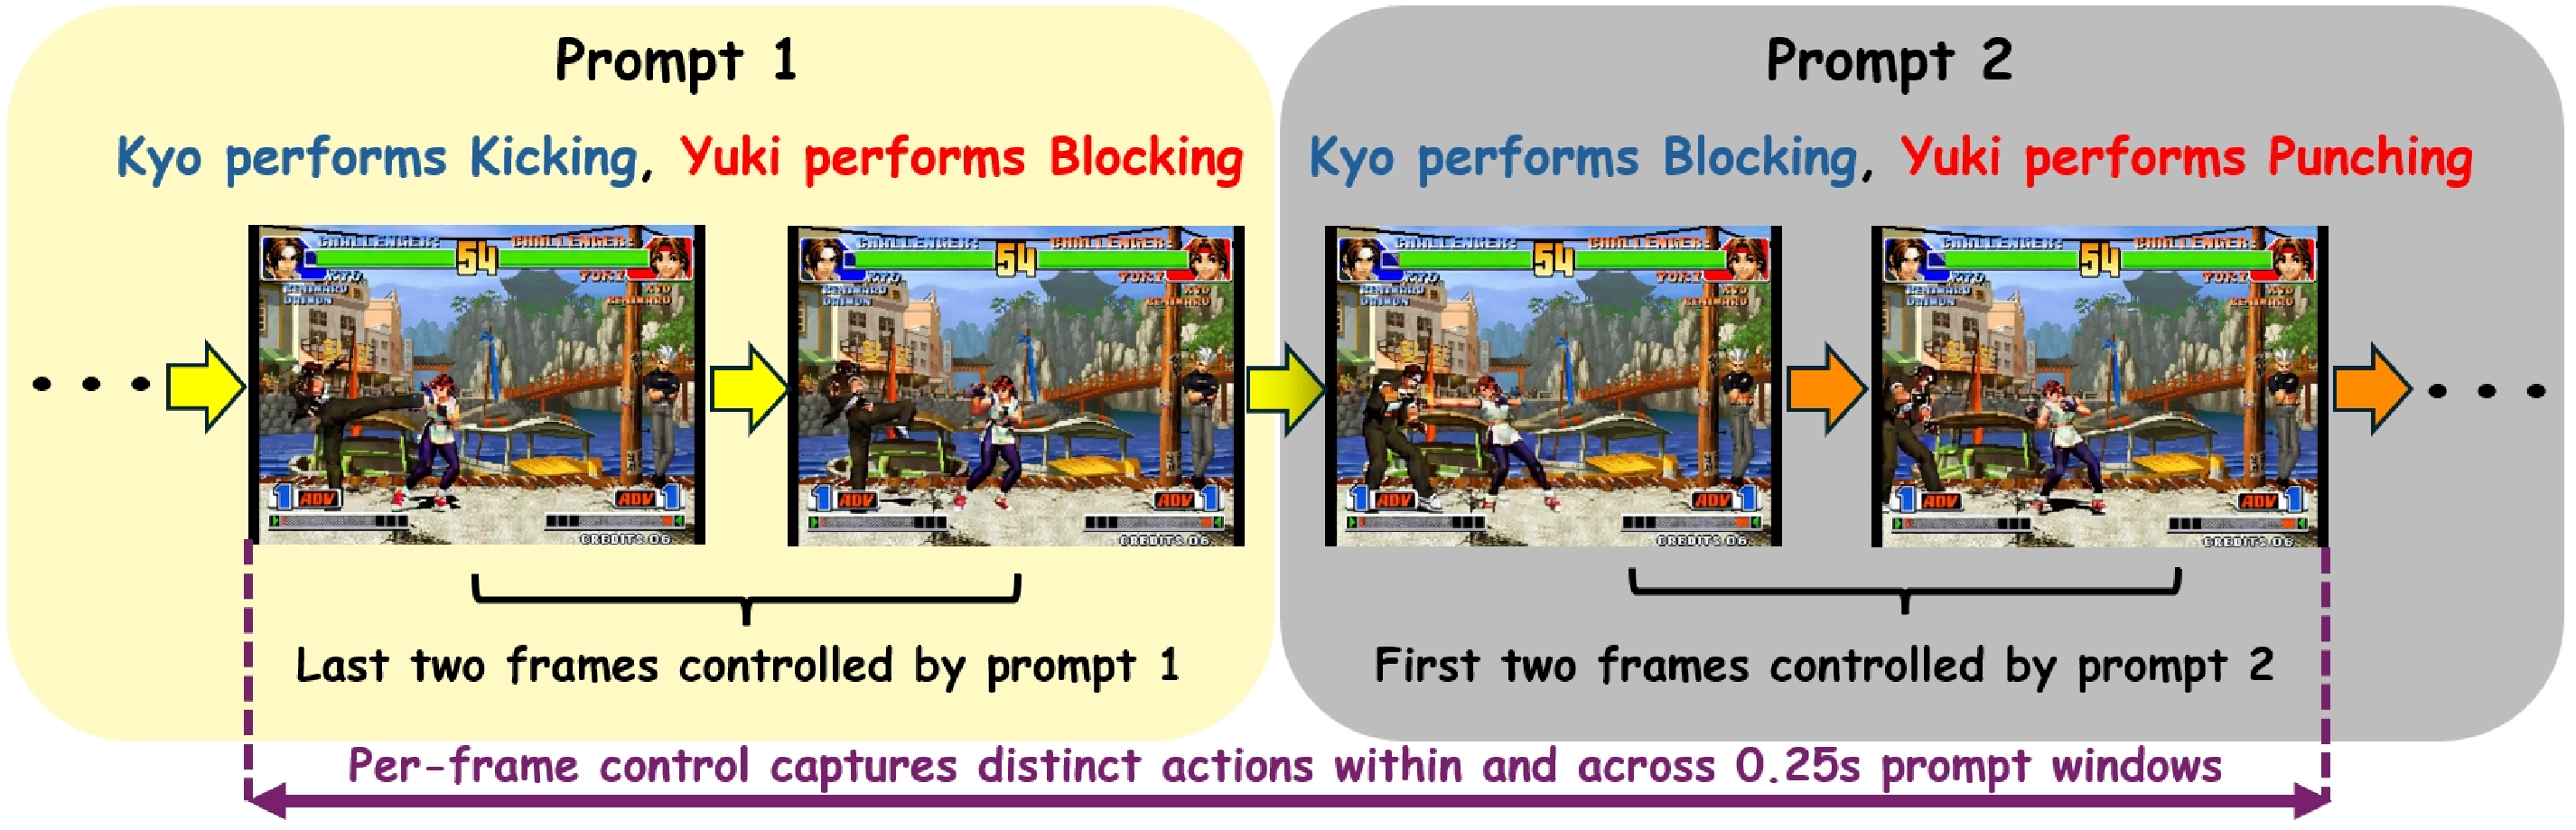
\includegraphics[width=\linewidth]{figures/fig_kof_demo.pdf}
% %     \caption{\textbf{Demonstrations of \methodname's fine-granularity multi-entity control in the game \textit{KOF}.}}
% %     \label{fig:kof_demo}
% % \end{figure*}


% % We have studied the action interface of interactive video world models as a first-class design choice and shown that replacing engine-internal animation namespaces and device-level inputs with per-frame, per-entity natural language unlocks capabilities that no prior interface can express. Under identical architecture, data, and compute, this single change of interface yields a $46$\,pp aggregate gap on cross-entity action transfer and a $90$\,pp structural gap on out-of-vocabulary prompts; the same architecture replicates these results on a second visually unrelated world by vocabulary substitution alone, and the two-step student sustains $\mathbf{2}$-hour rollouts at $0.16$\,s per frame on a single H100. Together, these findings indicate that, in the single-viewpoint multi-entity regime, the action interface, not the generative backbone, is the decisive bottleneck.

% % The cross-entity result is the most consequential. \methodname{} renders concepts on bodies that have never produced them: Margit wielding a light blade, the Crucible Knight executing a signature tail attack, conditioned on nothing but a textual phrase. This is \emph{concept-level} synthesis: the model recovers both the motion and the visual concept of an action from the compositional structure of language and the priors of a pretrained text encoder, with no reference motion of the target action on the recipient body. As a direct consequence, the expressible behaviours of an interactive video world model are no longer bounded by its training-time animation inventory, but by the open vocabulary of its language interface.

% % We see this as one step toward a more general question: can a single language interface serve as a unified action protocol across entities, worlds, and ultimately embodiments? The structural barrier we remove in the multi-entity video setting, the binding of action semantics to a fixed body and a fixed engine, is the same barrier that obstructs cross-embodiment action transfer in robotics, where an action defined on a human demonstrator cannot be issued to a robot arm with a different morphology. A controlled multi-entity video testbed of the kind we construct offers a concrete and quantitatively measurable environment for studying this question through a language interface, and we release our code, checkpoints, and $128$-hour frame-accurate per-entity action dataset to support work in this direction.

% % \paragraph{Limitations.} Open-vocabulary expressiveness is 
% % bounded by the pretrained text encoder: 
% % composing tokens already embedded in the encoder 
% % is straightforward, but truly novel concepts 
% % (neologisms or proper nouns absent from the encoder's 
% % training data) require encoder adaptation. 
% % Per-frame, per-entity action labels also assume some 
% % form of in-engine instrumentation; 
% % transferring the pipeline to environments without 
% % memory access (real-world video, closed-source engines) 
% % calls for an alternative annotation channel. 
% % Finally, our evaluation is on game worlds whose 
% % physical fidelity tolerance is set by the engine; 
% % extending the same interface to real-world embodied 
% % video generation will require additional treatment of 
% % physics, contact, and geometry. 
% % A complete discussion appears in Appendix~\ref{app:limitations}.

